% senior_thesis-proposal.tex
% CMPSC 580, Spring 2016
%
%
% This document provides a sample senior thesis proposal template for use
% by students in Allegheny's CS and Applied Computing programs.
%
%   *******************************************************************
%   * LOOK FOR BLOCK COMMENTS SUCH AS THIS ONE FOR AN EXPLANATION OF  *
%   * THIS DOCUMENT AND HOW TO MODIFY IT FOR YOUR OWN PROPOSAL!       *
%   *                                                                 *
%   * ANY LINE BEGINNING WITH A "%" IS A LATEX COMMENT AND IS IGNORED *
%   * BY THE LATEX PROCESSOR. YOU ARE ENCOURAGED TO COMMENT YOUR OWN  *
%   * LATEX CODE.                                                     *
%   *******************************************************************

%   ********************************************************************
%   * THE FIRST SECTION OF THE LATEX FILE IS THE "PREAMBLE." IT        *
%   * INSTRUCTS LATEX TO IMPORT SPECIAL PACKAGES FOR THINGS LIKE       *
%   * INCLUDING FIGURES, DOUBLE-SPACING, COLORED TEXT, ETC.            *
%   * DEPENDING ON YOUR NEEDS, YOU MAY FIND IT NECESSARY TO USE PACK-  *
%   * AGES THAT ARE NOT INCLUDED IN THIS TEMPLATE. SIMPLY IMITATE THE  *
%   * "\usepackage{...}" COMMANDS SHOWN BELOW.                         *
%   ********************************************************************

%   ********************************************************************
%   * BEGINNING OF PREAMBLE:                                           *
%   ********************************************************************
\documentclass[11pt]{article}

\usepackage[T1]{fontenc}
\usepackage{mathptmx}
\topmargin 0.0in
\setlength{\textwidth} {420pt}
\setlength{\textheight} {620pt} 
\setlength{\oddsidemargin} {20pt}
\setlength{\marginparwidth} {72in}

%   ********************************************************************
%   * Many of the commands below were simply copied over from an older *
%   * version of the proposal template; you can just leave them as     *
%   * they are (or you can delve into the TeX/LaTeX documentation      *
%   * and figure out what they do). Otherwise, jump ahead to the next  *
%   * block of comments, where you will enter title, abstract, etc.    *
%   ********************************************************************

\usepackage{fancyhdr} 
\usepackage{url}
\usepackage{graphicx}

% set it so that subsubsections have numbers and they
% are displayed in the TOC (maybe hard to read, might want to disable)

\setcounter{secnumdepth}{3}
\setcounter{tocdepth}{3}

% define widow protection

\def\widow#1{\vskip #1\vbadness10000\penalty-200\vskip-#1}

\clubpenalty=10000  % Don't allow orphans
\widowpenalty=10000 % Don't allow widows

% this should give me the ability to use some math symbols that 
% were available by default in standard latex (i.e. \Box)

\usepackage{latexsym}

% define a little section heading that doesn't go with any number

\def\littlesection#1{
\widow{2cm}
\vskip 0.5cm
\noindent{\bf #1}
\vskip 0.0001cm 
}

\pagestyle{fancyplain}

\newcommand{\tstamp}{\today}   
\renewcommand{\sectionmark}[1]{\markright{#1}}
\lhead[\Section \thesection]            {\fancyplain{}{\rightmark}}
\chead[\fancyplain{}{}]                 {\fancyplain{}{}}
\rhead[\fancyplain{}{\rightmark}]       {\fancyplain{}{\thepage}}
\cfoot[\fancyplain{\thepage}{}]         {\fancyplain{\thepage}{}}

\newlength{\myVSpace}% the height of the box
\setlength{\myVSpace}{1ex}% the default, 
\newcommand\xstrut{\raisebox{-.5\myVSpace}% symmetric behaviour, 
  {\rule{0pt}{\myVSpace}}%
}

% leave things with no spacing extra spacing in the final version of the paper
\renewcommand{\baselinestretch}{1.0}    % must go before the begin of doc

% suppress the use of indentation for a paragraph

\setlength{\parindent}{0.0in}
\setlength{\parskip}{0.1in}

\begin{document}


% handle widows appropriately
\def\widow#1{\vskip #1\vbadness10000\penalty-200\vskip-#1}

% build the title section

\makeatletter

\def\maketitle{%
  %\null
  \thispagestyle{empty}%
  %\vfill
  \begin{center}%\leavevmode
    %\normalfont
    {\Huge \@title\par}%
    %\hrulefill\par
    {\normalsize \@author\par}%
    \vskip .4in
%    {\Large \@date\par}%
  \end{center}%
  %\vfill
  %\null
  %\cleardoublepage

  }

\makeatother

%   ********************************************************************
%   * Here is the first place where you need to begin customizing:     *
%   * Enter you name, the title of your proposal, etc., in the places  *
%   * indicated by the comment "% CHANGE!".                            *
%   ********************************************************************

\vspace*{-1.1in}
\title{Title of Your Senior Thesis Proposal}  % CHANGE!

% build the author section
\author{
        Your Full Name\\  % CHANGE!
        Department of Computer Science\\
        Allegheny College \\
        {\tt youremail@allegheny.edu}  \\  % CHANGE!
        \url{http://www.cs.allegheny.edu/~yourwebsite/} \\  % CHANGE OR DELETE!
        \vspace*{.1in} \today \\ \vspace*{.1in}
}

\maketitle       % use the default title stuff

% Default "abstract" environment is too small; customize one instead:
\begin{center}
\large\bf Abstract
\vspace{-1em}  % Reduce space between header and the abstract
\end{center}

%   ********************************************************************
%   * Here is the second place where you need to customize:            *
%   * enter your abstract in the "quote" environment:                 *
%   ********************************************************************

\begin{quote}
The MuSic program takes biological sequences (DNA, RNA, Proteins, etc.), and represents the sequences (especially where the sequences align) with music. Sequence alignment tools are essential to biological research and may also be applied to align unknown sequences with other relevant known sequences \cite{}. The program offers a different way for scientist to pick up patterns and similarities in sequences just by listening to them. To translate this music into a visualization of the sequences, the visualizer would have to mainly account for timbre (sound color) and even the use of databases and manipulation of mp3 metadata (usually holds title, artist and other song information).
\end{quote}

%\vspace*{-.4in}
\section{Introduction}
\label{sec:introduction}
\vspace*{-.1in}

%   ********************************************************************
%   * Enter the text of your introductory section here.                *
%   ********************************************************************

The MuSic program represents the alignment of sequences correctly, through many harmonious, abstract, and unguided sounds. This begs the question, can we really expect everyone or anyone to pick up on all the different patterns going on in these abstract sounding songs? \\ \\
While the MuSic program may be good for certain musicians and biologists to study, there are many people who have trouble picking up on patterns in music. Being able to display these musical notes and sequences visually would provide a solution to those who have trouble hearing the aligned sequence patterns. This research will not implement a MuSic visualizing system. Instead it will explore how the musical sounds produced by MuSic are interpreted by a computer. Because there is no implementation in this project, this project serves more as a resource to the future of the MuSic visualizer and general music visualizers. In other words, our research will not narrow down how the visualizer should be implemented. Rather it will provide a list of viable methodologies and hopefully draw on some points which were overlooked in previous research. This research is essential to the future of this project, because it lays the foundation for how a computer would "hear" or interpret the biological sequences and then visualize them \cite{}. Future research can then build on the findings in this paper to implement a fully functioning visualization system. 

\vspace*{-.1in}
\section{Related Work}
\label{sec:relatedwork}
\vspace*{-.1in}

%   ********************************************************************
%   * Enter the text of your related work section here.                *
%   ********************************************************************

The previous research and published papers I will be building off of either pertains to research on the MuSic program, or to music visulazation in general. Table 1 shows the articles title, topic, and the main point our research will be using.\cite{conrad-gecco-selection-study}.
\begin{table}[htbp]
\centering
\begin{tabular}{|c||c|c|}
\hline
\bf Author & \bf Topic & \bf Main point\\\hline\hline
Ohmi, K & Music Visulization & Uneeded repetition in visualization systems\\\hline
Foote, J & Music Visualization & Graphical representation and retrival of music\\\hline
Ciuha, P & Music Visualization & Representing harmonies and relationships with colors\\\hline
Kubelka, O & Music Visualization & Preprocessed music visualization animation\\\hline
Zimmerman, F & Music Visualization & Graphically illustrating the tones, harmonies, tonalities, etc.\\\hline
Gerhard, D & Computer Music Analysis & Music decoding: easy. Music translation to a visual: difficult\\\hline
Smith, S & Computer Music Analysis & Computer hearing vs Human hearing, Timbre\\\hline
Burk, P & Computer Music Analysis & Understanding Timbre\\\hline
Chung, Y & The MuSic System & MuSic's applcation and importance\\\hline
\end{tabular}
\caption{Proposed work schedule}
\label{intro-tab1}
\end{table}

\vspace*{-.2in}
\section{Method of Approach}
\label{sec:method}
\vspace*{-.1in}

%   ********************************************************************
%   * Enter the text of your method of approach section here.          *
%   ********************************************************************

The first step of our methodology is to use a music production software to experiment with audio clips produced by the MuSic software. Specifically, we'll analyze the amplitude, frequency, and phase and applying useful tools and facts from previous research. After collecting this data from a variety of different sounding MuSic audio clips, we’ll analyze how effective our ideal method of breaking a polyphonic track into monophonic sounds works along with the use of a database to hold data. If we find our method problematic because of our experimental data or other unseen issues, we will suggest more suitable methods based off of previous research and other findings.

\vspace*{-.2in}
\section{Evaluation Strategy}
\label{sec:evaluate}
\vspace*{-.1in}

%   ********************************************************************
%   * Enter the text of your evaluation strategy section here.         *
%   ********************************************************************

Based of previous research we can use the fact that the same pitches share the same frequency, similar pitches share harmonics, wavelength patterns define timbre and can be used to identify instruments, and other facts about phase and amplitude to identify certain sounds \cite{} \cite{}. We will do this first with MuSic audio clips, and expand to simpler audio clips (for example a clip with only two or one main voices) if necessary. Our goal is to collect enough varying data (sounds high and low, short and fast vs. slow and long, polyphonic and monophonic), that we can effectively start to pick out visual aspects of the waves which differentiate sounds from one another. Because of harmonics unique relationship to certain notes, the use of harmonics to aid in the process is very likely \cite{}. If we can effectively differentiate the sounds by wavelength, we can then make a database of these different wavelength to sounds. This paves the way for an implementation using a music visualizer system.\\
We will analyze graphical representations such as the one below to compare different frequencies, wavelength patterns, phase, and amplitude.\\
\begin{figure}
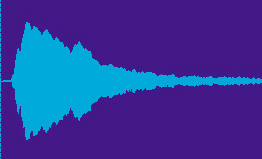
\includegraphics[scale=.2]{Music4}
\end{figure}
\begin{center}
Figure 1
\end{center}
While experimenting and observing, we will keep in mind that the attack, sustain, and decay (Figure 2) of the note all change how the music looks graphically in Figure 1 as well.
\begin{figure}
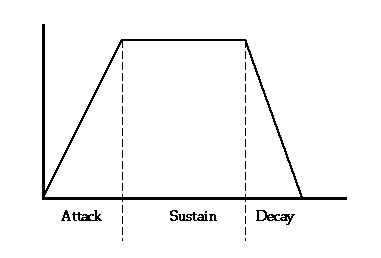
\includegraphics[scale=.2]{Music3}
\end{figure}
\begin{center}
Figure 2
\end{center}
After we've conducted our experiments and effectively picked up on patterns in frequency, wavelength, and other aspects of the wave, we will study the usefulness of visually representing whole songs similarly to the figure below. Specifically, the figure uses self-similarity to help point out patterns between the intro and outro (coda), verses, chorus', etc. \cite{}
\begin{figure}
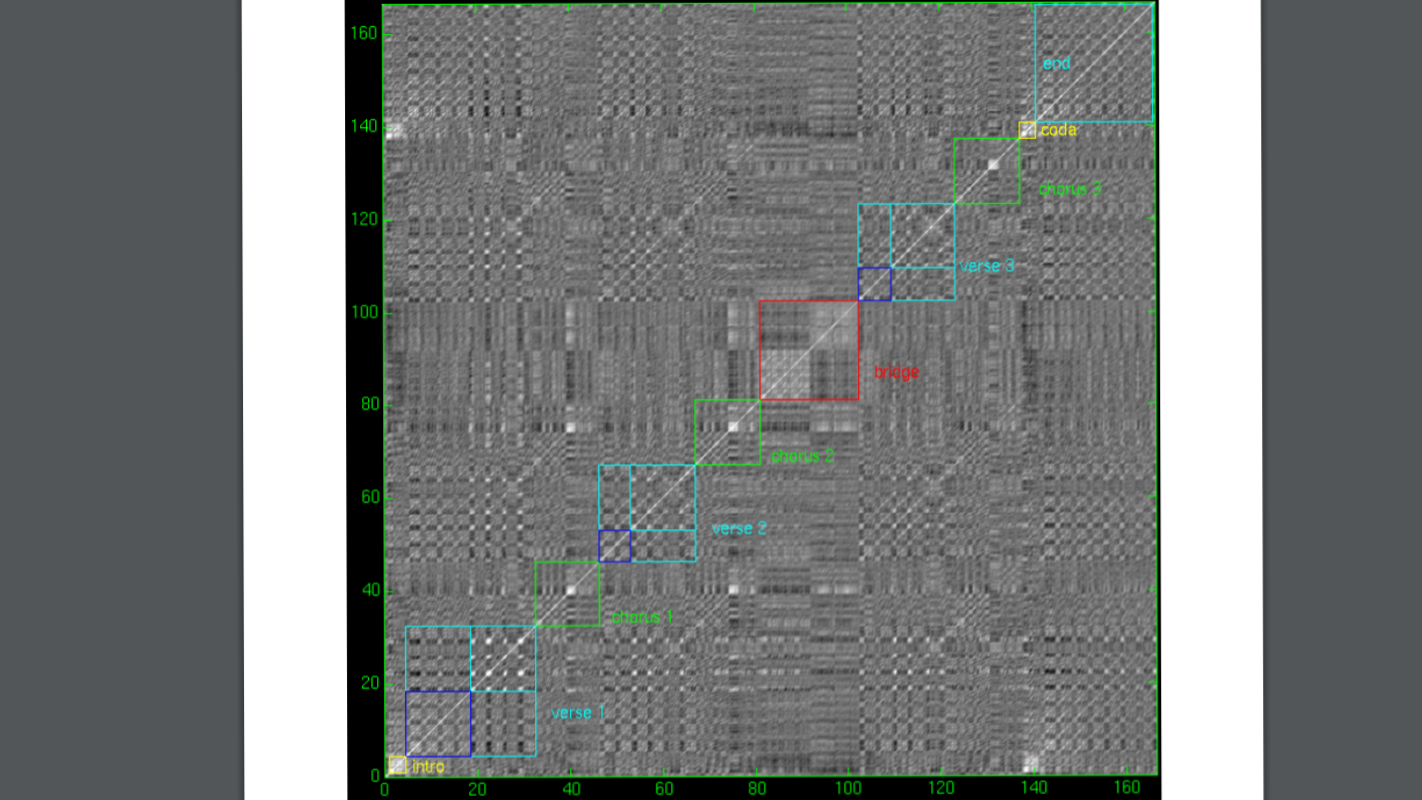
\includegraphics[scale=.2]{Music1}
\end{figure}
\begin{center}
Figure 3
\end{center}
Lastly, we will provide information about other aspects of visualization such as color choice based off of harmonies(shown in the figure below), and will touch on other subjects such as Pitch Tracking & Determination, Rhythm and Time, score generation, multi-pitch estimation, and will keep in mind know about how computers and people perceive music when working to visualize it.

\vspace*{-.1in}
\section{Research Schedule}
\label{sec:schedule}
\vspace*{-.1in}

\begin{table}[htbp]
\centering
\begin{tabular}{|c||c|c|}
\hline
\bf Task & \bf Begin Date & \bf End Date\\\hline\hline
First draft & Now & 27 Feb\\\hline
Second draft & 27 Feb & 6 Mar\\\hline
Third draft & 13 Mar & 20 Mar\\\hline
Fourth draft & 27 Mar & 4 Apr\\\hline
Fifth draft & 11 Apr & 18 Apr\\\hline
\end{tabular}
\caption{Proposed work schedule}
\label{intro-tab1}
\end{table}

\vspace*{-.1in}
\section{Conclusion}
\label{sec:conclusion}
\vspace*{-.1in}

%   ********************************************************************
%   * Enter the text of your concluding section section here.          *
%   ********************************************************************
In conclusion, this research will help further the MuSic tool which has already been proved to be "essential to biological research" \cite{}. It would expand the tools horizons, and if this research were not to happen, we would totally miss the opportunity to represent this tool which is so "essential to biological research" visually. This is not the only reason this research is crucial, but it also acts as a huge resource to anyone developing a music visualizing system. Because of this, it would be ignorant to put off a project with this much potential to affect the future of MuSic and music visualization.
 \cite{jia2011analysis}.

\bibliographystyle{plain}
\bibliography{senior_thesis_proposal}

\end{document}
